\documentclass[12pt]{scrartcl}
\usepackage[sexy]{evan}
\usepackage{graphicx,amsmath,amssymb,amsthm,amsfonts,babel}
\usepackage{tikz, tkz-euclide}
\usepackage{lipsum}
\usepackage{setspace}
\graphicspath{ {./} }
\usetikzlibrary{calc,through,intersections}
\usepackage[paperwidth=16cm, paperheight=16cm,margin=0.65cm]{geometry}

\colorlet{EvanRed}{Red!50!Purple}

\newcommand{\siku}[4][.5cm]
	{
	\coordinate (tempa) at ($(#3)!#1!(#2)$);
	\coordinate (tempb) at ($(#3)!#1!(#4)$);
	\coordinate (tempc) at ($(tempa)!0.5!(tempb)$);%midpoint
	\draw[black] (tempa) -- ($(#3)!2!(tempc)$) -- (tempb);
	}
	\usetikzlibrary{calc,positioning,intersections}

\setstretch{1.5}

\usepackage{etoolbox}
\newcommand{\zerodisplayskips}{%
  \setlength{\abovedisplayskip}{5pt}%
  \setlength{\belowdisplayskip}{5pt}%
  \setlength{\abovedisplayshortskip}{5pt}%
  \setlength{\belowdisplayshortskip}{5pt}}
\appto{\normalsize}{\zerodisplayskips}
\appto{\small}{\zerodisplayskips}
\appto{\footnotesize}{\zerodisplayskips}
\setlength\parindent{10pt}

\title{\vspace{-2cm}\textcolor{Red!80}{K}\textcolor{Green!80}{T}\textcolor{Blue!70}{O}\textcolor{YellowOrange!80}{M} Maret 2022}
\author{\vspace{-1.5cm}Isian no. 9 dan 12}
\date{\vspace{-0.4cm}Official problems (with original wording) and solutions by Azzam L. H.}


\begin{document}
\maketitle
\pagestyle{plain}
\vspace{-1.5cm}
\section{Soal}
\begin{enumerate}
\item Misalkan $N$ adalah banyaknya pasangan terurut himpunan $A$ dan $B$ yang memenuhi:
\begin{itemize}
\item $A \cup B = \{1,2,3,4,5,6,7,8,9,10\}$,
\item $\mathcal{A} \cap \mathcal{B} = \emptyset$,
\item $|A|$ bukan anggota $A$,
\item $|B|$ bukan anggota $B$.
\end{itemize}
Carilah nilai $N$. ( $|X|$ menotasikan banyaknya elemen himpunan $X$.)

\item Pada segiempat konveks $ABCD$ sisi $CD$ tegak lurus terhadap diagonal $AC$, sisi $AB$ tegak lurus terhadap diagonal $BD$, $CD = 130$, dan $AB = 56$. Titik $E$ adalah proyeksi titik $B$ terhadap $AD$. Jika $BE$ memotong diagonal $AC$ di $O$ dengan $AO = 16$ dan panjang $CO = x$, carilah $\left \lfloor x \right \rfloor$.
\end{enumerate}

\newpage
\section{Komentar (atau mungkin termasuk hint juga (?))}
\begin{enumerate}
\item[\textbf{No. 1}] Jika dilihat di soal, kita sebenarnya sudah diarahkan untuk mengobservasi apa yang terjadi antar dua himpunan $A$ dan $B$. Beberapa eksperimen kecil atau mencoba-coba beberapa nilai yang memenuhi untuk dimasukkan ke dalam $A$ atau $B$ mungkin akan membawa kita ke ide penyelesaian yang sebenarnya tidak terlalu sulit. Mungkin hanya butuh kesabaran dan sedikit nguli :).

\item[\textbf{No. 2}] Setelah membuat gambar dengan bagus, akan terlihat banyak sudut siku-siku (dan tentu saja segitiga siku-sikunya). Kalau seperti ini bisa dieksploitasi kesebangunan atau bisa kuli trigon habis-habisan. Setidaknya aku menemukan dua cara dengan bantuan trigon, jadi ya... ini soal trigon banget.

Di lain sisi, mungkin ada juga yang terpikir untuk membawa ke lingkaran (sadari bahwa $ABCD$ siklis dengan $AD$ adalah diameternya), tapi entah kenapa aku ngga nemu (baca: malas mengulik lagi) pake cara ini.
\end{enumerate}

\newpage
\section{Solusi}
\begin{proof}[\textbf{Solusi Nomor 1. }]
Partisi himpunan $\{1,2,\cdots,10\}$ menjadi dua himpunan, yaitu $A$ dan $B$ dengan $|A|=n$ dan $|B|=10-n$.

Karena $n$ bukan anggota $A$, maka haruslah $n$ anggota $B$ sehingga dengan ide yang sama $10-n$ haruslah anggota $A$. Perhatikan karena $A \cap B = \emptyset$, maka $n \neq 5$ karena jika $n=5$ maka $n \in A$ dan $n \in B$ yang jelas tidak mungkin. Lalu, jelas bahwa $n \neq 0$ karena $A \cup B = \{1,2,3,4,5,6,7,8,9,10\}$ sehingga 0 bukan anggota $A$ atau $B$.

Kita punya $\dbinom{8}{n-1}$ cara memilih elemen untuk $A$. Hal tersebut karena ada $n$ elemen di $A$ dan angka $10-n$ harus ada di $A$ (tidak boleh dipilih lagi karena sudah pasti di $A$) dan angka $n$ pasti ada di $B$ (tidak boleh dipilih lagi karena sudah pasti di $B$). Berarti hanya boleh $n-1$ angka ($n$ kemungkinan dikurangi 1 kemungkinan yang tidak boleh dipilih tersebut) yang dipilih dari $10-1-1=8$ (10 elemen total dikurangi 1 yang pasti di $A$ dan dikurangi 1 yang pasti di $B$) elemen sisanya.

Oleh karena itu banyaknya cara memilih pasangan terurut tersebut sama dengan banyak cara memilih kombinasi anggota untuk $A$, yaitu $$N=\left(\sum_{n=1}^{9} \dbinom{8}{n-1}\right) - \dbinom{8}{5-1}=2^{8}-70= \boxed{186}.$$

\end{proof}

\begin{proof}[\textbf{Solusi Nomor 2.}]

Misalkan $\angle CAD=\alpha$ dan $\angle BDA=\beta$. Karena $\angle AEB = \angle ABD$ dan $\angle EAB = \angle BAD$ maka $\triangle ABE$ dan $\triangle ADB$ sebangun sehingga didapat $\angle ABE=\angle ADB=\beta$.

\begin{center}
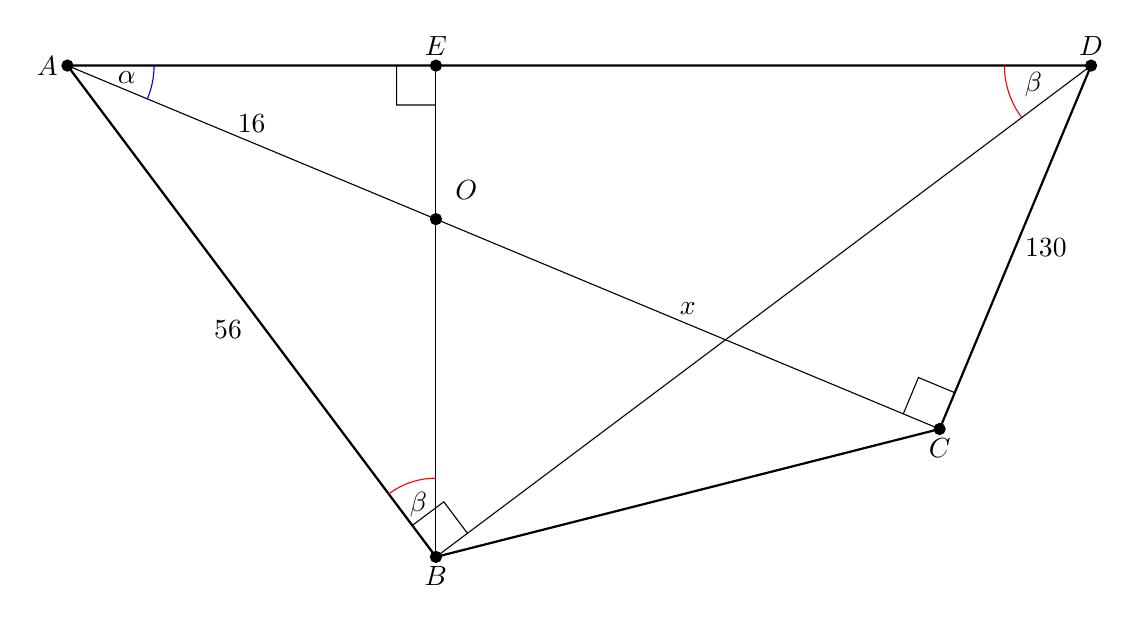
\begin{tikzpicture}[scale=1]
    \coordinate[label=left:$A$] (A) at (0,0);
    \coordinate[label=above:$D$] (D) at (13,0);
    \coordinate[label=above:$E$] (E) at (4.68,0);
    \coordinate[label=below:$B$] (B) at (4.68,-6.24);
    \coordinate[label=below:$C$] (C) at (11.077,-4.6154);
    \draw[thick] (D)--(A)--(B)--(C)--cycle;
    \draw[name path=BE] (B)--(E);
    \draw[name path=AC] (A)--(C);
    \draw (D)--(B);
    \path[name intersections={of=AC and BE,by=O}];
    \node[label=above right:$O$] at (O) {};  
    \path (A)--(O) node[above, midway]{$16$};
    \path (O)--(C) node[above, midway]{$x$};   	
    \siku{A}{B}{D}
    \siku{A}{C}{D}
    \siku{A}{E}{B}
    \pic[draw=red,angle radius=1.1cm,pic text=$\beta$,angle eccentricity=.7] {angle={A--D--B}};
    \pic[draw=red,angle radius=1cm,pic text=$\beta$,angle eccentricity=.7] {angle={E--B--A}};
    \pic[draw=blue,angle radius=1.1cm,pic text=$\alpha$,angle eccentricity=.7] {angle={C--A--D}};
    \foreach \s in {D,A,B,C,E,O} \filldraw (\s) circle (2pt);
    \path (D)--(C) node[right,midway]{$130$};
    \path (B)--(A) node[below left,midway]{$56$};
\end{tikzpicture}
\end{center}

Kita punya $AE=AB\sin \angle ABE=56\sin\beta$ dan $AE=AO \cos \angle EAO=16\cos\alpha$ sehingga didapatkan
\begin{align}
56\sin\beta = 16\cos\alpha . \label{eq:1}
\end{align}

Selanjutnya $AD=\dfrac{DC}{\sin \angle DAC}=\dfrac{130}{\sin\alpha}$ dan $AD=\dfrac{AB}{\sin \angle ADB}=\dfrac{56}{\sin\beta}$ yang mengakibatkan
\begin{align}
\dfrac{130}{\sin\alpha}=\dfrac{56}{\sin\beta} \Rightarrow 130\sin\beta=56\sin\alpha. \label{eq:2}
\end{align}

Dengan membagi persamaan \eqref{eq:2} dengan persamaan \eqref{eq:1} didapat

\begin{align*}
\dfrac{130\sin\beta}{56\sin\beta}=\frac{56\sin\alpha}{16\cos\alpha} 
\Rightarrow \frac{130}{56}=\frac{7}{2}\tan\alpha 
\Rightarrow \tan\alpha=\frac{65}{98}
\end{align*}
Oleh karena itu didapatkan bahwa, $CA=\dfrac{CD}{\tan\alpha}=\dfrac{130}{\frac{65}{98}}=196$, sehingga $x=CO=CA-AO=180 \implies \left \lfloor x \right \rfloor = \boxed{180}$.
\end{proof}
\end{document}